\begin{figure}
    \centering
    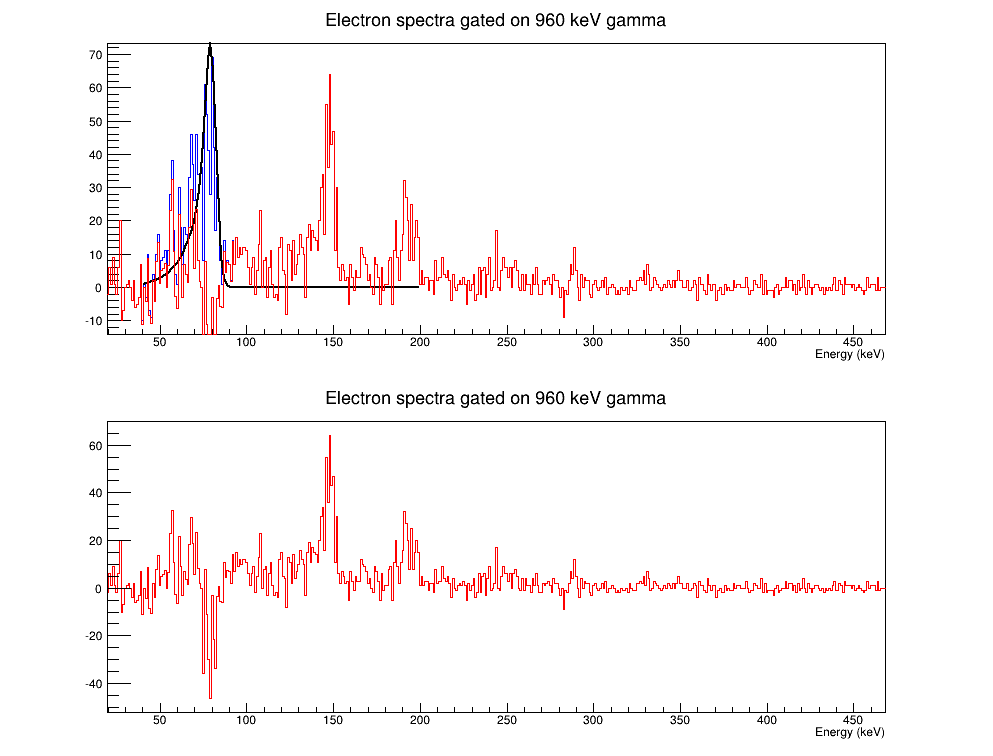
\includegraphics[scale=0.4]{Analysis_Figs/Subtraction_SiLiAll_960.png}
    \caption[An example of the subtraction used to removed the ground state band peaks from spectra.]{An example of the subtraction used to removed the ground state band peaks from spectra. To subtract the conversion electron peak off, the area of the corresponding gamma peak was taken from the same gate. Using the conversion coefficient and the efficiencies of both detectors, the area of the peak could be calculated. From there, this value, along with fixed $R$, $\beta$, $\sigma$, and centroid were used to subtract the peak off. The black line is the function used for subtraction. The blue line is the original spectrum, and the red liine is after subtraction. This code can be found in Appendix \ref{chap:macro}}
    \label{fig:subtraction}
\end{figure}